\documentclass[10pt,a4paper]{article}

\usepackage[utf8]{inputenc}
\usepackage[T1]{fontenc}

\usepackage{amsmath,mathtools,amsfonts,amssymb}
\usepackage{graphicx}
\usepackage[spanish]{babel}
\usepackage{lastpage,tabto,xcolor}
\usepackage[a4paper, top=0.8in, bottom=1in, left=0.7in, right=0.7in]{geometry}
\usepackage{fancyhdr}
\usepackage{comment}
\usepackage{multicol}
\usepackage{titling} % Para ajustar los espacios del título
\usepackage{tasks} % Para listas en columnas
\usepackage{tikz}
\usepackage{pgfplots}
\pgfplotsset{width=7cm,compat=1.15}
\usepackage{caption}

% Fecha de versión automática según fecha de compilación
\newcommand{\verdate}{\the\year.\ifnum\month<10 0\fi\the\month.\ifnum\day<10 0\fi\the\day}

% Ajusta la separación entre el encabezado y el contenido
\setlength{\headsep}{10pt}

% Ajuste del título: 
\setlength{\droptitle}{-0.5in} % Mueve el título ligeramente hacia arriba
\pretitle{\begin{center}\vspace{-1em}\normalfont\Large}
	\posttitle{\par\end{center}\vspace{-4em}}
\preauthor{\begin{center}\vspace{-0.5em}}
	\postauthor{\par\end{center}}
\predate{}\postdate{}

\pagestyle{fancy}
\lhead{\footnotesize Análisis de Señales y Sistemas  - Año \the\year{} Ver. \verdate}
\rhead{\footnotesize Trabajo Práctico N$^\text{o}$3: Sistemas de tiempo continuo.}
\rfoot{\footnotesize Página \thepage\ de \pageref{LastPage}}
\renewcommand{\headrulewidth}{0.4pt}
\renewcommand{\footrulewidth}{0.4pt}

% Título optimizado con espacios reducidos
\title{%
	{\normalsize Departamento de Ingeniería en Tecnologías Electrónicas, UTN FRM}\\[0.1cm]
	{\large Análisis de Señales y Sistemas}\\[0.15cm]
	{\normalsize Trabajo Práctico N$^{\text o}$3: Sistemas de tiempo continuo}%
}
\author{}
\date{}


\begin{document}
	\maketitle
	\thispagestyle{fancy}
	
	% Entorno de dos columnas
	\begin{multicols}{2}
		
		\label{sec:enun}
		% ***********************************************
			\textbf{Generalidades sobre sistemas}
			\begin{enumerate}
			% ***********************************************
			% 				Ejercicio 1
			% ***********************************************
			\item {Determinar la linealidad de los siguientes sistemas:}
			\begin{enumerate}
				\item $ y(t) = \cos [x(t)] $
				\item $ y(t) = t^2x(t-1) $
			\end{enumerate}
			
			% ***********************************************
			% 				Ejercicio 2
			% ***********************************************
			\item {Considerar un sistema con relación entre su entrada $x(t)$ y salida $y(t)$ dada por $y(t)=tu(t)x(t)$. Determinar si el sistema es invariante en el tiempo y justificar la respuesta.}
			
			% ***********************************************
			% 				Ejercicio 3
			% ***********************************************
			\item{Determinar la linealidad e invariancia en el tiempo de los siguientes sistemas:}
			\begin{enumerate}
				\item $y(t)=\sin{[x(t)]}$
				\item $y(t)=[x(t)]^2$
			\end{enumerate}
			
			% ***********************************************
			% 				Ejercicio 4
			% ***********************************************
			\item {Determinar la linealidad, invariancia en el tiempo y causalidad del siguiente sistema:}
			\begin{enumerate}
				\item $y(t)=x\left(\frac{1}{2}t\right)$
			\end{enumerate}
			
			% ***********************************************
			% 				Ejercicio 5
			% ***********************************************
			\item {Demostrar que el sistema descripto por la relación $y(t)=x(t-6)-x(1-t)$, es lineal y no causal.}
			
			% ***********************************************
			\textbf{Convolución de señales}
			% ***********************************************
			% 				Ejercicio 6
			% ***********************************************
			\item Dadas las señales de entrada $x(t)$ y respuesta impulsiva $h(t)$, 
				determinar la salida del sistema $y(t)$.
			
			\begin{center}
				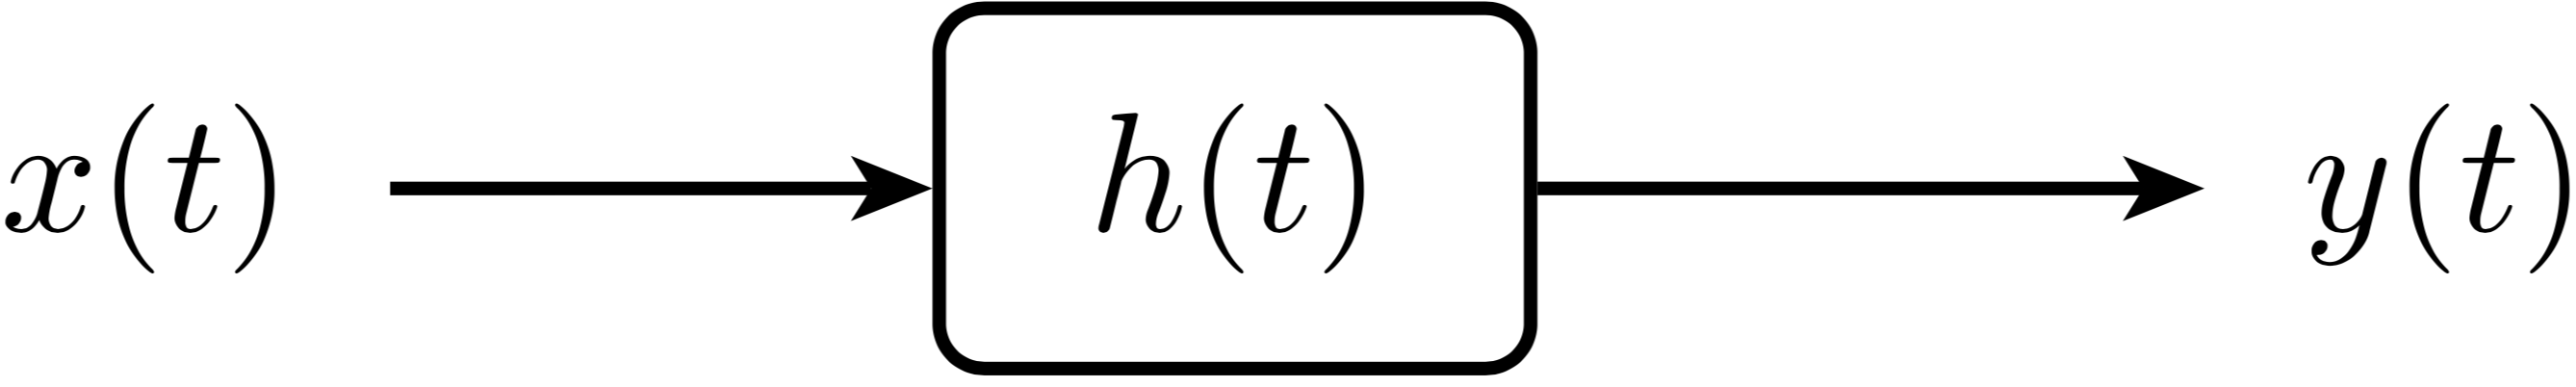
\includegraphics[width=0.6\linewidth]{figures/fig_ej6/tp6-pics_sistema1.png}
			\end{center}
			
			\begin{enumerate}
				\item $x(t)=e^{-3t}u(t)~;~h(t)=e^{-\frac{1}{2}t}u(t)$
				\item $x(t)=(t+1)u(t)~;~h(t)=e^{-2t}u(t)$
				\item $x(t)=tu(t)~;~h(t)=\cos{(3t)}u(t)$
			\end{enumerate}
			
			% ***********************************************
			% 				Ejercicio 7
			% ***********************************************
			\item {Obtener la convolución entre $h(t)=e^{-t}u(t)u(5-t)$ y $x(t)=tu(t)u(3-t)$ aplicando la definición.}
			
			% ***********************************************
			% 				Ejercicio 8
			% ***********************************************
			\item {Determinar $y(t)=x(t)*h(t)$, siendo:}
			
			$x(t)=
			\begin{cases}
			1, & ~0\leq t\leq 1, \\
			0, & ~t<0~ \vee t>1,
			\end{cases}$
			~~ y ~~
			$h(t)=
			\begin{cases}
			t, & ~0\leq t\leq 2, \\
			0, & ~t<0~ \vee t>2.
			\end{cases}$
			
			% ***********************************************
			\textbf{Interconexión de sistemas LIT}
			% ***********************************************
			% 				Ejercicio 9
			% ***********************************************
			\item Para cada par de sistemas LIT con respuestas al impulso $h_1(t)$ y $h_2(t)$, determinar la respuesta al impulso equivalente cuando se los conecta en cascada y en paralelo.
			\begin{enumerate}
				\item $h_1(t)=e^{-t}u(t)~;~h_2(t)=\delta(t-2)$
				\item $h_1(t)=u(t)-u(t-1)~;~h_2(t)=u(t)-u(t-1)$
				\item $h_1(t)=\delta(t)-\delta(t-T)~;~h_2(t)=u(t)$
			\end{enumerate}

			% ***********************************************
			\textbf{Propiedades de los sistemas LIT}
			% ***********************************************
			% 				Ejercicio 10
			% ***********************************************
			\item ¿Cuáles de las siguientes respuestas al impulso corresponden a sistemas estables LIT? ¿Son sistemas causales?
			\begin{enumerate}
				\item $h(t)=e^{-(1-2j)t}u(t)$
				\item $h(t)=e^{2t}\cos(3t)u(t+1)$
				\item $h(t)=e^{-t}\sin(2t)u(t)$
			\end{enumerate}

			% ***********************************************
			% 				Ejercicio 11
			% ***********************************************
			\item Sobre la relación entre la respuesta al impulso $h(t)$ y la respuesta al escalón $g(t)$ de un sistema LIT:
			\begin{enumerate}
				\item Dado $h(t)=e^{-2t}u(t)$, calcular la respuesta al escalón $g(t)$ aplicando $g(t)=\int_{-\infty}^{t}h(\tau)\,d\tau$ y graficar el resultado.
				\item Dada la respuesta al escalón de un circuito $RC$, $g(t)=(1-e^{-t/\tau_0})u(t)$ con $\tau_0=RC$, recuperar la respuesta al impulso $h(t)$ por derivación.
				\item Sea $h(t)=\delta(t)-\delta(t-T)$ con $T>0$. Calcular $g(t)$, graficarla e identificar la operación que el sistema realiza sobre la entrada.
			\end{enumerate}

			% ***********************************************
			\textbf{Sistemas descritos por ecuaciones diferenciales}
			% ***********************************************
			% 				Ejercicio 12
			% ***********************************************
			\item Para cada una de las siguientes ecuaciones diferenciales que vinculan la entrada $x(t)$ con la salida $y(t)$, determinar si el sistema (con condiciones iniciales en reposo) es lineal e invariante en el tiempo. Justificar.
			\begin{enumerate}
				\item $\dot{y}(t)+3y(t)=2x(t)$
				\item $\dot{y}(t)+t\,y(t)=x(t)$
				\item $\dot{y}(t)+y^2(t)=x(t)$
				\item $\ddot{y}(t)+4\dot{y}(t)+3y(t)=\dot{x}(t)+x(t)$
			\end{enumerate}

			% ***********************************************
			% 				Ejercicio 13
			% ***********************************************
			\item Construir el diagrama en bloques de la realización directa con derivadores de los siguientes sistemas, indicando explícitamente las ganancias de cada rama.
			\begin{enumerate}
				\item $\dot{y}(t)+3y(t)=2x(t)$
				\item $\ddot{y}(t)+4\dot{y}(t)+3y(t)=x(t)$
			\end{enumerate}

		\end{enumerate}
		
	\end{multicols}

\end{document}
